 \documentclass{report}
 
\usepackage[utf8]{inputenc} 
\usepackage[T1]{fontenc}      
\usepackage[top=3.5cm, bottom=3cm, left=3.0cm, right=4.0cm]{geometry}
\usepackage{graphicx}
\usepackage{amsmath,esint }
\usepackage{amssymb}
\graphicspath{{figures/}{../figures}}

\begin{document}

\section*{Machines de Carnot et de Stirling}

On considère une machine thermodynamique effectuant les transformations suivantes, sur un gaz parfait contenant $n$ moles : 

\begin{itemize}
\item[•]$A \rightarrow B$ : compression isotherme, réversible à la température $T_f$ (contact avec une source froide)
\item[•]$B \rightarrow C$ : compression adiabatique, réversible
\item[•]$C \rightarrow D$ : détente isotherme, réversible à la température $T_c$ (contact avec une source chaude)
\item[•]$D \rightarrow A$ : détente adiabatique, réversible

\end{itemize}

Ce cycle est appelé cycle de Carnot, qui permet en théorie, d'obtenir un rendement maximal. On supposera que le rapport des volumes $V_A/V_B=10$. Questions : 

\begin{itemize}

	\item[$\clubsuit$] Tracer le cycle dans un diagramme de Clapeyron. Ce cycle est-il moteur ou récepteur ? Justifier. 

	\item[$\clubsuit$] Déterminer, pour chaque transformation, $\Delta U$, $W$, et $Q$. 
	
	\item[$\clubsuit$] En déduire le rendement théorique.
	
\end{itemize}

On s'intéresse au cycle de Stirling, dans lequel les transformations $B \rightarrow C$ et $D \rightarrow A$ sont désormais des isochores au contact respectivement de la source chaude et source froide. Les autres transformations sont les mêmes. Le cycle de Stirling a l'avantage de pouvoir être réalisable en pratique sur des dispositifs appelés \textit{moteurs de Stirling}, contrairement au cycle de Carnot, théorique.

\begin{itemize}

	\item[$\spadesuit$] Mêmes questions que pour le cycle de Carnot ci-dessus. Quel est le rendement théorique ? Montrer qu'il est nécessairement inférieur au rendement de Carnot.
	
	\item[$\spadesuit$]	 Montrer que l'on peut récupérer une partie d ela chaleur lors du cycle pour atteindre le rendement de Carnot.
	
	\item[$\spadesuit$] On suppose qu'une voiture normale est mue par le moteur étudié jusque-là. En supposant que la chaleur apportée par la source chaude est créée par de la combustion d'essence, de pouvoir calorifique de 35 475kJ.L$^{-1}$. Estimer la quantité d'essence injectée à chaque cycle ? Combien vaut alors $T_c$ ?
	
%\item[4-] Application numérique : calculer le rendement dans ce cas-là. On prendra $V_A/V_B=10$.
\end{itemize}

\newpage

\section*{Cycle de Beau de Rochas}

Les moteurs à essence équipant la plupart des véhicules terrestres sont des machines thermodynamiques constitués de un ou plusieurs cylindres, dans lequels un piston fait subir sur $n$ moles de gaz parfait le cycle suivant (dit de Beau de Rochas) :

\begin{itemize}

\item[$A \rightarrow B$ :] compression adiabatique, réversible du volume $V_A$ au volume $V_B$ : le mélange d'air et essence est comprimé ;
\item[$B \rightarrow C$ :] échauffement isochore en contact de la source chaude, en pratique il s'agit de la combustion très rapide de l'essence ;
\item[$C \rightarrow D$ :] détente adiabatique, réversible du volume $V_B$ au volume $V_C=V_A$ : les gaz de combustion "poussent" le cylindre en fournissant du travail ;
\item[$D \rightarrow A$ :] refroidissement isochore en contact de la source froide : les gaz issus de combustion sont évacués et remplacés par par un mélange d'air frais et d'essence.

\end{itemize}

Ce cycle de fonctionnement a l'avantage de pouvoir faire varier la puissance rapidement en faisant varier à la demande la quantité de chaleur $Q_c$ apportée par l'essence lors de la transformation $B \rightarrow C$, mais au détriment du rendement. On souhaite montrer que le rendement $\eta$ de ce cycle est nécessairement inférieur au rendement de Carnot $\eta_C$.

\begin{itemize}

	\item[$\clubsuit$] Décrire ce cycle dans un diagramme de Clapeyron et justifier qu'il est moteur.

	\item[$\clubsuit$] Déterminer, pour chaque transformation, $\Delta U$, $W$, et $Q$ en fonction de températures $T_A$, $T_B$, $T_C$ et $T_D$ atteintes aux moments $A$, $B$, $C$ et $D$.
	
	\item[$\clubsuit$] Déterminer les tempratures $T_B$, $T_C$ et $T_D$ en fonction de $T_A$. Quel paramètre doit-on introduire pour calculer $T_C$ ? 
	
	\item[$\clubsuit$]  Calculer son rendement $\eta$ en fonction de $a=V_A/V_B$ et $\gamma$. 
	
	\item[$\clubsuit$] Rappeler le rendement de Carnot $\eta_C$ et montrer que celui-ci est nécessairement supérieur au rendement $\eta$ de ce cycle.
	
	\item[$\clubsuit$] On suppose que ce moteur sert à mouvoir une voiture individuelle. En supposant que la chaleur apportée par la source chaude est créée par de la combustion d'essence, de pouvoir calorifique de 35 475kJ.L$^{-1}$; estimer le volume d'essence injecté à chaque cycle. Combien vaut alors $T_c$ ?
	
\end{itemize}

\textit{Données : $ V_{2}/V{1} = 10$ et $ \gamma=1.4$}

\newpage

\section*{Exercice 2}

On étudie l'écoulement d'un gaz dans une tuyère horizontale isolée thermiquement du milieu extérieur.

En régime permanent, dans une section droite de la tuyère les vitesses d'écoulement sont égales et normales à la section. La pression et la température sont indépendantes du temps et uniformes :
\begin{itemize}
\item[-]à l'entrée de la tuyère, $x=x_{1}$ : $P_{1} = 3$ bars; $T_{1} = 300$ K;
\item[-]à la sortie de la tuyère, $x=x_{2}$ : $P_{2} = 1$ bars; $T_{2} = 250$ K
\end{itemize}

Soit $H_{m}(x)$ l'enthalpie molaire du gaz à l'abscisse $x$ et $M$ la masse molaire du gaz. 

\begin{itemize}
\item[•] Montrer que pour une mole de gaz passant dans la tuyère, on peut écrire $H_{m}(x)+\frac{1}{2}Mv^{2}(x)= cste$.
\item[•] On suppose que $v(x_{1})$ négligeable, calculer $v(x_{2})$. On supposera le gaz parfait. 
\end{itemize}

\textit{Données : $M = 32g.mol^{-1}$ et $\gamma=1.4$}

\begin{figure}[!h]
\centering
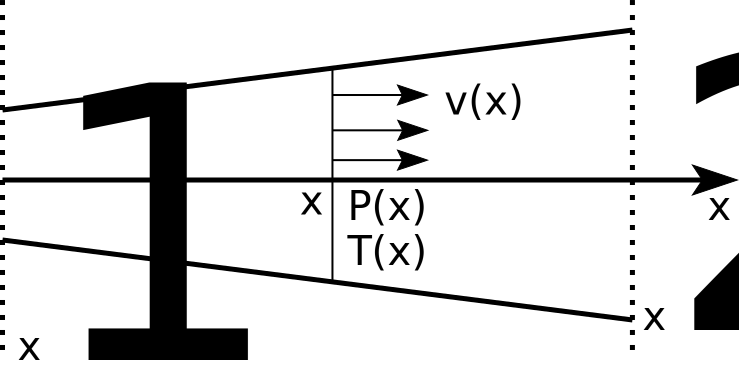
\includegraphics[width=0.4\linewidth]{turbine.pdf}
\end{figure}

\subsubsection*{Étude d'une turbine}
On suppose que le gaz est utilisé à la sortie pour actionner une turbine située dans la tuyère. A l'entrée, il a une vitesse $v_{2}$, une température $T_{2}$ et une pression $P_{2}$. A la sortie, la pression et la température sont inchangées, mais la vitesse est nulle. 
\begin{itemize}
\item[•] Calculer le travail récupéré par la turbine lors du passage d'une mole de gaz.

\end{itemize}

\subsubsection*{Étude d'une fusée}

On suppose désormais que la tuyère est celle d'un propulseur spatial, équipant une fusée de masse $M_0$ à vide, contenant une masse $m_0$ de gaz carburant. Le gaz est stocké sous pression à une température initiale $T_1$ et est éjecté à une température $T_2$. On négligera les différences entre le cas où la tuyère est horizontale ou verticale et toute force de frottement sur la fusée. 

\begin{itemize}
	\item[•] Comment relier la vitesse d'éjection des gaz $v_2$ avec la variation de la vitesse $\frac{d}{dt} V(t)$ de la fusée ? 
	\item[•] Quelle est la vitesse de la fusée lorsque tout le gaz a été éjecté ?
\end{itemize}

\newpage

\section*{Exercice 3}

\subsection*{Premier principe}

Une ampoule de volume de $V_1$, dans laquelle règne le vide, est entourée d'air ambiant à la pression $P_{0} = 1$atm et à la température $T_{0}=20^{\circ}C$, qu'on assimile à un gaz parfait de coefficient $\gamma=1.4$. On perce un petit trou dans l'ampoule, l'air s'y engouffre et au bout d'une durée très courte, la pression dans l'ampoule est égale à la pression ambiante.

Quel est la température $T_{1}$ dans l'ampoule une fois celle-ci remplie?

\begin{figure}[!h]
\centering
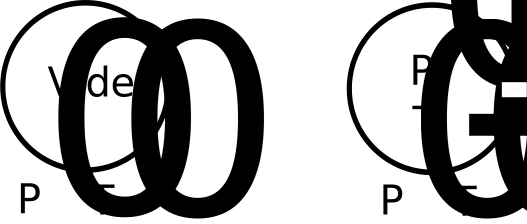
\includegraphics[width=0.5\linewidth]{ampoule.pdf}
\end{figure}

\section*{Second principe}

Soit un système de volume constant constitué d'un nombre $N>>1$ de particules en équilibre à la température T et dont chacune peut avoir deux niveau d'énergie $E_{1}$ et $E_{2}$, avec $E_{1}<E_{2}$.

Soit $n_{1}$ le nombre de particules dans l'état d'énergie $E_{1}$ et $n_{2}$ le nombre de particules dans l'état d'énergie $E_{2}$.

On suppose que la répartition des particules se fait selon la loi de Boltzmann :
\begin{equation}
\frac{n_{2}}{n_{1}}=exp\left( \frac{E_{2}-E_{1}}{k_{b}T}\right) 
\end{equation}

Cette distribution indique que les niveaux ont d'autant plus de chance d'être peuplés qu'ils n'ont pas une énergie élevée. D'autre part plus la température est élevée, plus les niveaux d'énergies élevées pourront être peuplés. 

\begin{itemize}
\item[-]Déterminez la différentielle de l'énergie interne du système en fonction de $n_{1}$ et $E_{2}-E_{1}$.
\item[-]On rappelle que l'entropie peut s'écrire comme $S=k_B\ln\Omega$, où $\Omega$ est le nombre de configurations possibles pour le système. Exprimez $S$ en fonction de $N$ et $n_1$. On utilisera la formule de Stirling $\ln (N!)=N \ln (N)$ valable pour $N>>1$.
\item[-] Exprimez la différentielle de $S$ en fonction de $T$, $\Delta$ et $n_1$.
\item[-] Montrez que l'on retrouve l'identité thermodynamique : $dU = TdS$
\end{itemize}

\newpage

\section*{Exercice 4}

Dans tout le problème, les échanges de travail et de chaleur seront toujours considérés du point de vue du gaz.
\begin{itemize}

\item[•] On considère le réfrigérant représenté ci-dessous, qu'on suppose parfaitement calorifugé. Le gaz, de chaleur massique $c_{p}$ est refroidi à pression constante, de la température $T_{2}$ à la température $T_{3}$, au moyen d'un circuit d'eau (de chaleur massique $c$ constante), qui, elle, est réchauffée de $t_{0}$ à $t_{1}$.

\begin{figure}[!h]
\centering
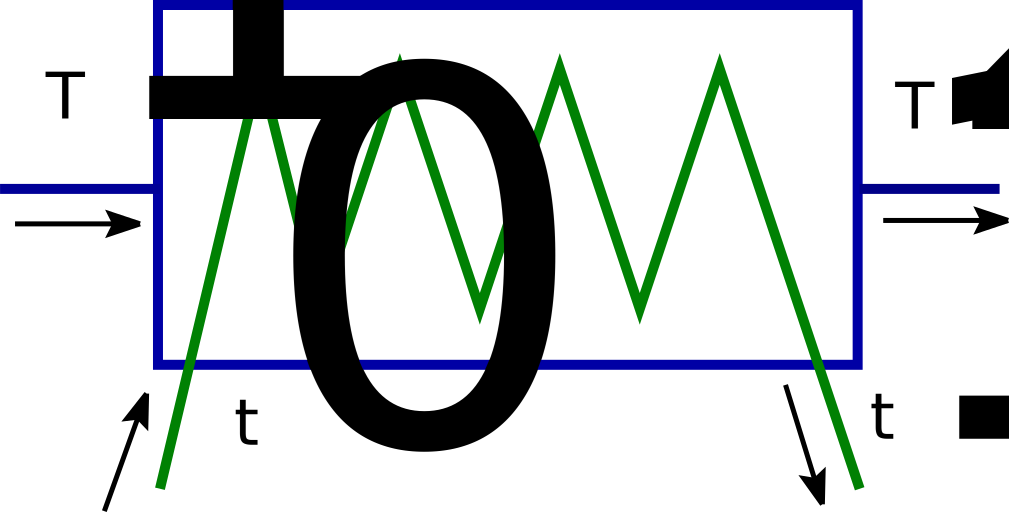
\includegraphics[width=0.3\linewidth]{refrigirant.pdf}
\end{figure}

Le débit massique du gaz étant imposé, déterminer le débit massique $D$ nécessaire du circuit d'eau de refroidissement.
\item[•] On considère maintenant un échangeur de chaleur représenté ci-dessous. Il comporte deux canalisations dans lesquelles le même gaz circule avec le même débit mais dans des sens opposés. Les températures d'entrées, supposées connues, seront notées $T_{4}$ et $T_{9}$ et les température de sorties respectives $T_{5}$ et $T_{10}$. Dans chaque canalisation, la pression est constante.
\begin{figure}[!h]
\centering
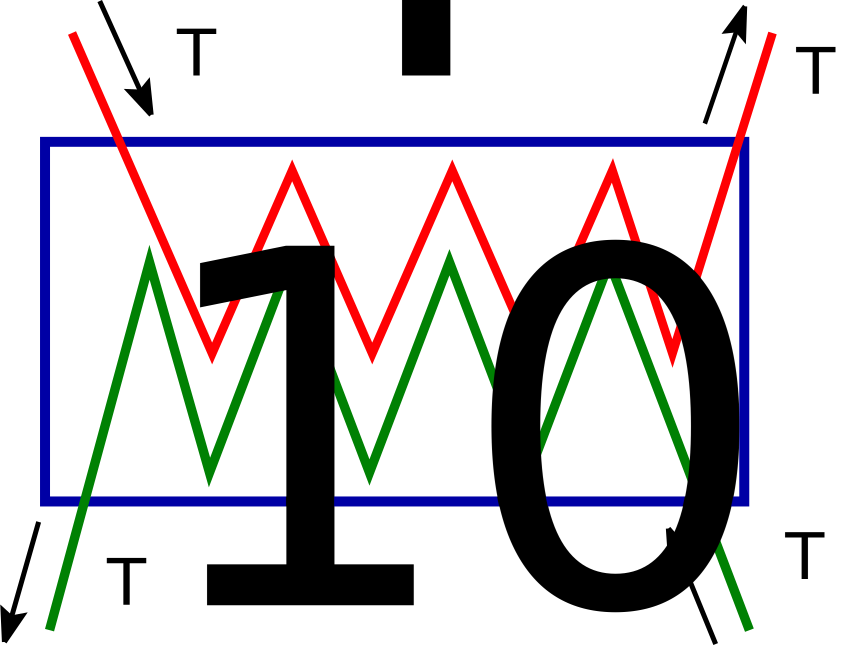
\includegraphics[width=0.3\linewidth]{echangeur.pdf}
\end{figure}
On suppose d'abord réversible les transformations subies par le gaz dans chaque canalisation. En utilisant les fonctions enthalpie et entropie, écrire les relations reliant $T_{5}$ et $T_{10}$ à $T_{4}$ et $T_{9}$.

En déduire les solutions physiquement acceptables pour $T_{5}$ et $T_{10}$.

Si les transformations sont en fait irréversibles, quel les inégalités satisfaites par $T_{5}$ et $T_{10}$, si l'on suppose $T_{4}>T_{9}$ ?

\item[•] On définit l'efficacité comme étant : $e=\frac{T_{5}-T{4}}{T_{9}-T{4}}$ en considérant la canalisation 4-5. Montrer qu'on obtient la même efficacité en considérant la canalisation 9-10.
\end{itemize}

\newpage

\section*{Exercice 5}

\begin{figure}[!h]
\centering
\includegraphics[width=0.4\linewidth]{thermo2.pdf}
\end{figure}

On considère un fil de caoutchouc décrit par les variables d'état suivantes : sa longueur $L$, sa température $T$ et $F$ la force appliquée dessus. On le modélise à travers une équation d'état de la forme : 
\begin{equation}
	F(L,T) = F_0 + \rho(L-L_0) + \sigma(T-T_0)
\end{equation}
où $\rho$ et $\sigma$ sont des constantes positives et les grandeurs indicées par "0" sont des grandeurs intrinsèques au fil. D'autre part, on admet que l'énergie interne du fil s'écrit : 
\begin{equation}
	U(L,T) = C_L(T-T_0)+(F_0-\sigma T_0)(L-L_0) +\frac{ \rho}{2}(L-L_0)^2 +U_0
\end{equation}
où $C_L$ est une constante. 

On attache désormais le fil de caoutchouc en $CM$, où le cercle de centre $O$ et de rayon $OM=R$ tourne à la vitesse angulaire $\omega$. On a $CO=a\ll R$. Le cercle est plongé à son diamètre entre deux source de chaleurs à températures $T_1$ et $T_2$  (avec $T_1>T_2$) :

\begin{figure}[!h]
\centering
\includegraphics[width=0.3\linewidth]{thermo3.pdf}
\end{figure}

En tournant dans le sens de rotation indiqué sur le schéma, le fil subit les transformations successives suivantes :
\begin{itemize}
\item[$A\rightarrow B$ :] Une transformation isotherme à $T_1$ lorsque le fil est dans la demi-partie supérieure (rouge)
\item[$B\rightarrow C$ :] Lorsque le fil passe à l'horizontale (longueur $R-a$), il passe instantanément de $T_1$ à $T_2$
\item[$C\rightarrow D$ :] Une transformation isotherme à $T_2$ lorsque le fil est dans la demi-partie inférieure (bleue)
\item[$D\rightarrow A$ :] Lorsque le fil passe à l'horizontale (longueur $R+a$), il passe instantanément de $T_2$ à $T_1$
\end{itemize}
Questions : 
\begin{itemize} 
\item[$\spadesuit$] Par analogie avec le travail des forces de pression d'un gaz parfait ($P, V\leftarrow F, L$), montrer que le travail reçu par l'élastique sur une transformation $A\rightarrow B$ s'écrit $W=\int_A^B dL\cdot F$.
\item[$\spadesuit$] Décrire le cycle dans un diagramme de Clapeyron $(F,L)$.
\item[$\spadesuit$] Calculer les divers échanges mécaniques et thermiques au cours de ce cycle.
\item[$\spadesuit$] Le cycle proposé est-il moteur ? Calculer son rendement.
\end{itemize}

\newpage

\section*{Exercice 6}

On considère un cylindre rempli d'un gaz parfait à la température $T_1$, à la pression $P_1$ et un volume $V_1=aS$, où $a$ est la hauteur et S la section.

Le cylindre est surmonté d'un piston, de masse $m$, libre de coulisser sans frottement. La pression à l'extérieur du dispositif est $P_0$.

Les parois du cylindre et du piston sont considérées comme athermane : il n'y a aucun échange thermique avec l'extérieur.

A un certain moment, on fait tomber une masse $M$ sur le piston d'une hauteur $H$. Après quelques oscillations, le piston retourne à un nouvel équilibre.


\begin{figure}[!h]
\centering
\includegraphics[width=0.5\linewidth]{thermo4.pdf}
\end{figure}

\begin{itemize}
\item[•] Calculez les paramètres internes du gaz au nouvel équilibre. 
\item[•] Pour quelle hauteur de chute $H_C$ le piston se retrouve t-il exactement à la même hauteur initiale $a$ ?
\item[•] Que se passe t-il si $M$ devient très lourde ?
\end{itemize}

\newpage

\section*{Exercice 7}

On considère le dispositif ci-dessous. Le piston (gris, entouré de noir) et les parois (en gris) sont adiabatiques. La paroi interne séparant les espaces $A$ et $B$ est fixe et diatherme. Elle est percée d'un trou fermé par une fenêtre amovible. La pression extérieure est $P_0=1$ bar. Initialement, le volume $B$ est rempli d'une mole de gaz parfait $\gamma=1,4$, avec une pression $P_0=1$ bar, une température $T_0=300$K. Le volume $A$ est vide.

\begin{figure}[!h]
\centering
\includegraphics[width=0.5\linewidth]{thermo1.pdf}
\end{figure}

\begin{itemize}
\item[•] On ouvre la fenêtre. Décrire qualitativement ce qu'il se passe suivant le volume de $A$. En déduire l'existence d'un volume critique $V_C$ que l'on ne demande pas de calculer ici.

\item[•] On suppose $V_A<V_C$. Déterminez l'état final du gaz en fonction de $(P_0, V_A, V_B)$. Calculer la création d'entropie. Quelle est la cause de la création d'entropie ? Déterminez $V_C$.

\item[•] On suppose désormais que $V_A>V_C$. Quel est l'état final ?

\end{itemize}

\newpage

\section*{Travail maximal de deux réservoirs finis}

On considère deux réservoirs $A$ et $B$ remplis du même gaz parfait caractérisé par $\gamma$, l'un contenant $n_A$ moles à la température $T_A$, l'autre $n_B$ moles à la température $T_B$. Ils sont parfaitements isolés du monde extérieur, mais peuvent échanger de la chaleur avec une machine thermique $M$, considérée comme parfaite (pas de capacité calorifique propre, pas de d'échange thermique autre qu'avec $A$ et $B$, aucun frottement). Cette machine peut néanmoins extraire un travail $W$ avec l'extérieur. 

\begin{itemize}
\item[$\blacklozenge$] Quelle est la quantité maximale de travail $W$ que peut extraire la machine $M$ ?
\end{itemize}

\newpage

\section*{Formation du brouillard}

On considère un gaz parfait de coefficient $\gamma$ contenu dans un cylindre de section $S$ orienté verticalement. L'altitude le long de ce cylindre est notée $z$, et on note $g$ l'accélération de la pesanteur supposée uniforme le long du cylindre. Le gaz est soumis à un mouvement ascendant dans le cylindre en se déplaçant à la vitesse notée $c$. Les parois du cylindre ne permettent pas de transfert thermique. L'écoulement est de plus supposé stationnaire.

On note $T_0$, $P_0$ et $c_0$ la température, la pression et la vitesse du gaz à l'altitude $z=0$ et $T(z)$, $P(z)$ et $c(z)$ ces trois grandeurs à l'altitude $z$. De la même manière, on introduit $h_{m,0}$ et $h_m(z)$ l'enthalpie massique du gaz à l'altitude $z=0$ et $z$.

\begin{itemize}
	
	\item[$\triangle$] En utilisant le premier principe industriel appliqué au gaz dans le cylindre entre les altitudes $z=0$ et $z$, trouver une relation entre $h_{m,0}$, $h_m(z)$, $c_0$, $c(z)$ et $z$.
	
	\item[$\triangle$] Pour simplifier le problème, on considère que la vitesse du gaz est quasi-nulle, de sorte à ce que $c_0=c(z)=0$. Montrer que la température obéit alors à la loi suivante :
	\begin{align*}
		T(z)=T_0(1-\frac{z}{H})
	\end{align*}
	Expliciter $H$ en fonction de $\gamma$, $g$ et la masse molaire du gaz $M$. Donner une estimation numérique.
	
\end{itemize}

On considère que le gaz étudié est de l'air humide, subissant une ascension verticale, lente et isentropique dans ce cylindre. La vapeur d'eau contenue en faible quantité dans l'air se comporte comme un gaz parfait. La pression de vapeur saturante de l'eau, notée $P_s$ et exprimée en Pa est une focntion de $T$ suivant la loi empirique suivante :
\begin{align*}
	\ln(P_s(T)) = a -\frac{b}{T}
\end{align*}

\begin{itemize}
	
	\item[$\triangle$] Soit $\varphi$ la fraction molaire de vapeur d'eau contenue dans une masse d'air ascendante. Après avoir explicité la pression $P(z)$ dans la colonne, déterminer la pression partielle $P_e(z)$ de cette vapeur. 
	
	\item[$\triangle$] A quelle altitude, notée $z_1$, peut-on avoir le changement d'état liquide-vapeur ? On pourra supposer que $z\ll H$.
	
	\item[$\triangle$] Justifier que les reliefs sont propices à l'apparition du brouillard.
	
\end{itemize}

\newpage	

\section*{Etude d'un turborécteur}

Un turboréacteur est un moteur thermique équipant les avions dits \textit{à réaction}, schématisé ci-dessous. Le fonctionnement général est le suivant : une turbine aspire et comprime l'air en amont du réacteur (soufflante et compresseur, étapes $1\rightarrow2$ et $2\rightarrow3$), qui est échauffé par la combustion du kérosène dans la chambre de combustion (étape $\rightarrow4$). Les gaz de combustion sont ensuite détendus ($4\rightarrow5$) à travers une turbine dont l'arbre est commun avec celui du compresseur et de la soufflante, puis ces gaz sont finalement évacués par la tuyère ($5\rightarrow6$), en accélérant fortement, fournissant la poussée requise.

Le but de l'exercice est de calculer la vitesse de sortie $c_6$ des gaz de combustion. On ne s'intéresse ici qu'au flux primaire, circulant dans le compresseur. Le flux dit secondaire, passant de $2\rightarrow7$ n'est pas étudié ici. 

\begin{figure}[!h]
\centering
	\includegraphics[width=0.65\linewidth]{turboreacteur.png}
\end{figure}

On formule les hypothèses suivantes pour les différentes transformations :
\begin{itemize}

	\item[$1\rightarrow3$ :] Soufflante et compresseur, compression adiabatique réversible au taux de compression $P_2/P_1=2$ puis $P_3/P_2=13$ ;
	\item[$3\rightarrow4$ :] Chambre de combustion, le gaz est chauffé jusqu'à $T_4=1450$K de manière isobare ;
	\item[$4\rightarrow5$ :] Détente adiabatique réversible du gaz de $P_4$ et $P_5$ à travers la turbine ;
	\item[$5\rightarrow6$ :] Détente adiabatique réversible du gaz de $P_5$ et $P_6$ dans la tuyère.

\end{itemize}

On supposera que le régime est stationnaire, que l'énergie potentielle de pesanteur du fluide est négligeable dans toutes les étapes. L'énergie cinétique sera aussi négligée dans toutes les étapes, sauf à la sortie de la tuyère (en 6) où le gaz est très fortement accéléré. On négligera tout frottement mécanique. Les pressions en entrée et en sortie sont $P_1=P_6=1$ bar et la température en entrée est $T_1=288$K. On note $C_p$ la capacité thermique massique de l'air.

\begin{itemize}

	\item[$\bigstar$] En s'inspirant de la démonstration du premier principe indutriel, montrer que le travail massique utile reçu par le gaz lors de la trasformation de l'état $i$ à $j$ (sauf pour $3\rightarrow4$, dans la chambre de combustion) est donné par :
	\begin{align*}
		w_{i\rightarrow j}=C_p(T_j-T_i) + \frac{1}{2}\left(c_j^2-c_i^2 \right) 
	\end{align*}
	
	\item[$\bigstar$] Donner une relation entre $P_i$, $P_j$, $T_i$, $T_j$ et $\gamma$ (sauf pour $3\rightarrow4$).
	\item[$\bigstar$] En exploitant le couplage mécanique entre turbine, compresseur et soufflante, établir les expressions littérales et les valeurs numériques des températures $T_2$, $T_3$, $T_5$ et de la pression $P_5$ en sortie de turbine.
	\item[$\bigstar$] En déduire la vitesse $c_6$ en sortie de turbine. 

\end{itemize}

\textit{Données :} $C_p=1,0\times10^3$J.kg$^{-1}$.K$^{-1}$, $\gamma=1,4$

\end{document}
